\section{Method}
\label{sec:method}

% Three-attentions schematic. Compiles with tikz (verify on first build).
\begin{figure}[t]
\centering
\begin{tikzpicture}[
  font=\small,
  box/.style={draw, rounded corners, minimum height=7mm, align=center, inner sep=3pt},
  enc/.style={box, fill=blue!8},
  att/.style={box, fill=orange!12},
  ar/.style={-{Latex[length=2mm]}, thick},
  node distance=5mm and 7mm]

\node[box, fill=gray!8] (fields) {event\\fields};
\node[enc, right=of fields] (evt) {Event\\Encoder\\{\scriptsize(attn 1)}};
\node[att, right=of evt] (hist) {History\\Encoder\\{\scriptsize(attn 2)}};
\node[box, right=of hist, fill=green!8] (head) {head};
\node[right=4mm of head] (out) {$\hat{y}$};

\draw[ar] (fields) -- (evt);
\draw[ar] (evt) -- (hist) node[midway,above,font=\scriptsize] {[EVT]};
\draw[ar] (hist) -- (head) node[midway,above,font=\scriptsize] {record emb.};
\draw[ar] (head) -- (out);

% cross-sequence (third attention) below
\node[box, fill=gray!8, below=9mm of evt] (nbr) {last-$K$ neighbour\\events at shared\\entity (other accts.)};
\node[att, right=of nbr, minimum height=10mm] (xseq)
  {Cross-Sequence Encoder\\{\scriptsize the third attention (attn 3)}};
\draw[ar] (nbr) -- (xseq);
\draw[ar, dashed] (nbr.north) to[out=90,in=180] (evt.west|-nbr.north) ;
\draw[ar] (evt.south) to[out=-90,in=180] ([yshift=2mm]xseq.west);
\draw[ar] (xseq.north) to[out=90,in=-90] (hist.south)
  node[midway,right,font=\scriptsize] {$+$ residual};

\begin{scope}[on background layer]
\node[draw, dotted, rounded corners, fit=(nbr)(xseq), inner sep=3pt, label={[font=\scriptsize]below:relational (cross-account)}] {};
\end{scope}
\end{tikzpicture}
\caption{A standard FFM has \emph{two} attentions: over an event's fields (Event Encoder) and over
an account's own history (History Encoder). We add a \emph{third}: a Cross-Sequence Encoder that
attends over a shared entity's recent events from \emph{other} accounts, encoded by the same Event
Encoder, and adds the result as a residual to the target's record embedding.}
\label{fig:arch}
\end{figure}


\subsection{The two-attention FFM backbone}
\label{sec:method:backbone}
We reproduce a standard FFM at laptop scale ($\approx$\num{10}M parameters).

\paragraph{Tokenisation.} Each event (a transaction, click, or page view) is a set of
$(\textrm{field},\textrm{value})$ pairs. Categorical values are mapped to per-field vocabularies;
numeric values (e.g.\ amount) are discretised into learned buckets; two calendar fields (hour of
day, day of week) are derived from the event timestamp. A learned \texttt{[EVT]} token is prepended
to each event's token set.

\paragraph{Two attentions.} An \textbf{event encoder} --- a set transformer with no positional
encoding --- contextualises an event's field tokens and returns its \texttt{[EVT]} vector, a
per-event embedding. A \textbf{history encoder} --- a bidirectional transformer with rotary
positional encoding~\cite{su2021roformer} on \emph{continuous event time} --- runs over an account's
sequence of \texttt{[EVT]} vectors and returns a record embedding $h_t$ per event. These are the two
attentions: within an event, and across an account's own history.

\paragraph{Pretraining.} We pretrain with masked modelling: a fraction of $(\textrm{field},
\textrm{value})$ tokens are masked and reconstructed by per-field heads, a self-supervised objective
requiring no labels. Concretely the backbone has $d_{\text{model}}{=}\num{256}$, \num{8} attention
heads, feed-forward width \num{1024}, and a context window of \num{128} events. We train each
dataset's backbone for \num{30000} steps with AdamW~\cite{loshchilov2019adamw}, a peak learning rate
of \num{3e-4}, \num{500} warm-up steps and cosine decay, batch size \num{128}, in \texttt{bf16} on a
single NVIDIA L40S GPU. Figure~\ref{fig:loss} shows the masked-modelling loss plateauing on every
dataset, confirming the backbone is converged before any adaptation.

% Pretraining learning curves — masked-modelling loss vs step, one line per dataset backbone.
\begin{figure}[t]
\centering
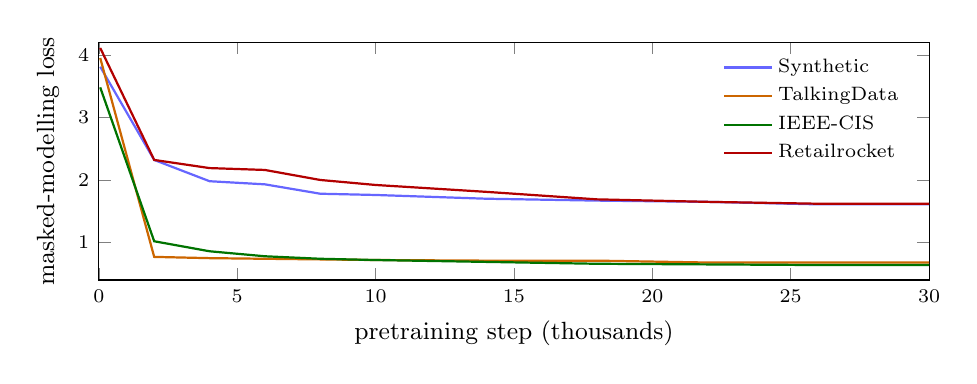
\begin{tikzpicture}
\begin{axis}[width=\linewidth, height=4.6cm,
  xlabel={pretraining step (thousands)}, ylabel={masked-modelling loss},
  xlabel near ticks, ylabel near ticks, xmin=0, xmax=30, ymin=0.4, ymax=4.2,
  legend style={font=\scriptsize, at={(0.98,0.98)}, anchor=north east, draw=none, fill=none},
  legend cell align=left, tick label style={font=\scriptsize}, label style={font=\small}]
\addplot[blue!60, thick] coordinates {(0.05,3.81)(2,2.32)(4,1.98)(6,1.93)(8,1.78)(10,1.76)(14,1.70)(18,1.67)(22,1.65)(26,1.61)(30,1.61)};
\addlegendentry{Synthetic}
\addplot[orange!80!black, thick] coordinates {(0.05,3.95)(2,0.77)(4,0.75)(6,0.74)(10,0.72)(14,0.71)(18,0.71)(22,0.68)(26,0.68)(30,0.68)};
\addlegendentry{TalkingData}
\addplot[green!45!black, thick] coordinates {(0.05,3.48)(2,1.02)(4,0.86)(6,0.78)(8,0.74)(10,0.72)(14,0.69)(18,0.66)(22,0.65)(26,0.64)(30,0.64)};
\addlegendentry{IEEE-CIS}
\addplot[red!70!black, thick] coordinates {(0.05,4.11)(2,2.32)(4,2.19)(6,2.16)(8,2.00)(10,1.92)(14,1.81)(18,1.69)(22,1.65)(26,1.62)(30,1.62)};
\addlegendentry{Retailrocket}
\end{axis}
\end{tikzpicture}
\caption{Masked-modelling pretraining loss for each dataset's backbone. Every curve plateaus well
before \num{30000} steps, so each FFM is converged before any adaptation.}
\label{fig:loss}
\end{figure}


\subsection{The third attention: a cross-sequence encoder}
\label{sec:method:xseq}
A per-account model never sees a shared entity's cross-account state. We add a third attention that
supplies exactly this. For a target event on account $a$ at shared entity $e$ (merchant, IP, item)
and time $t$, with record embedding $q{=}h_t\in\mathbb{R}^d$ from the history encoder, we gather the
neighbour set $\mathcal{N}_{e,t}=\{$the last $K$ events at $e$ with time strictly ${<}\,t\}$ ---
causal, across \emph{all} accounts, $|\mathcal{N}_{e,t}|\le K$. Each neighbour event $j$ is encoded
by the \emph{shared} event encoder $E$ into its \texttt{[EVT]} token, to which we add a learned
recency embedding of its lag:
\begin{equation}
\mathbf{z}_j \;=\; E(x_j) + \rho\!\big(\log(t-t_j)\big).
\end{equation}
An optional shallow transformer $T$ mixes the $K$ neighbours, $\{\mathbf{n}_j\}=T(\{\mathbf{z}_j\})$.
The target \emph{queries} them by multi-head cross-attention with a padding mask $m_j$ ($0$ for a
real neighbour, $-\infty$ for padding):
\begin{align}
Q &= W_Q\,q,\quad K_j = W_K\,\mathbf{n}_j,\quad V_j = W_V\,\mathbf{n}_j,\\
\alpha_j &= \operatorname{softmax}_j\!\Big(\tfrac{Q^{\top}K_j}{\sqrt{d_h}} + m_j\Big),\qquad
u = \textstyle\sum_j \alpha_j\,V_j .
\end{align}
The attention output is used only when the target has at least one in-window neighbour, so an
empty neighbourhood contributes an exact zero rather than a masked-softmax NaN:
\begin{equation}
p \;=\; \mathbb{1}\!\left[\mathcal{N}_{e,t}\neq\varnothing\right]\cdot
\operatorname{LayerNorm}\!\big(W_O\,u\big).
\end{equation}
Alongside the attention path, the encoder carries an always-on readout of a precomputed,
causal windowed velocity $c\in\mathbb{R}^{d_c}$ of the shared entity (the log count of prior
same-entity events within fixed time windows), projected and added:
\begin{equation}
\operatorname{xseq}(q,\{\mathbf{n}_j\},c) \;=\; p \;+\; \operatorname{LN}\!\big(\operatorname{GELU}(W_c\,c)\big),
\qquad h_t' = h_t + \operatorname{xseq} .
\end{equation}
The result is a residual added to the target's record embedding, which the head then reads
(Algorithm~\ref{alg:xseq}). The two internal paths --- attention over raw neighbours and the velocity
readout --- are complementary; we treat the module as a single unit and leave a formal decomposition
of their contributions to future work. Neighbours are the most recent $K$ prior events at $e$
(temporal recency, not similarity selection); their embeddings are recomputed each step so gradients
flow into the shared encoder. Throughout we use $K{=}\num{16}$, one mixing layer, and $d_c{=}\num{2}$
velocity windows.

\begin{algorithm}[t]
\caption{Cross-sequence attention for one target event}
\label{alg:xseq}
\begin{algorithmic}[1]
\Require target embed.\ $q{=}h_t$, entity $e$, time $t$, velocity $c$, window $K$; shared encoder $E$
\State $\mathcal{N} \gets$ last $K$ events at $e$ with time ${<}\,t$ \Comment{causal, all accounts}
\If{$\mathcal{N}=\varnothing$} \State $p \gets \mathbf{0}$
\Else
  \For{$j \in \mathcal{N}$} \State $\mathbf{z}_j \gets E(x_j) + \rho(\log(t-t_j))$ \EndFor
  \State $p \gets \operatorname{LN}\!\big(W_O\,\operatorname{MHA}(q,\,T(\{\mathbf{z}_j\}))\big)$
\EndIf
\State \Return $h_t + p + \operatorname{LN}(\operatorname{GELU}(W_c\,c))$
\end{algorithmic}
\end{algorithm}

\subsection{Adaptation strategies}
\label{sec:method:adapt}
We evaluate three ways to adapt the pretrained backbone to a binary target, plus the tabular baseline
below. All read the target event's final record embedding with a single linear head
($\mathbb{R}^{d}\!\to\!\mathbb{R}$) and train a class-weighted binary cross-entropy over as-of-date
windows (a window ending at each target event, no future leakage), with AdamW at learning rate
\num{3e-4}, \texttt{bf16}, a single seed.
\begin{itemize}
\item \textbf{Linear probe.} The backbone is \emph{frozen}; only the linear head is trained. This
measures what masked pretraining already preserved.
\item \textbf{Fine-tune.} The backbone is unfrozen and trained end-to-end with the head. This lets
the task reshape the two-attention representation.
\item \textbf{Fine-tune $+$ cross-attention.} The third attention (\S\ref{sec:method:xseq}) is added
and the whole model --- backbone, cross-sequence encoder, and head --- is fine-tuned end-to-end from
the same checkpoint. The cross-sequence encoder's weights are randomly initialised (it is not part of
pretraining) and learned during adaptation.
\end{itemize}
We fine-tune for \num{8} epochs on the synthetic data and \num{6} on the larger real corpora, with
batch size \num{128} (synthetic) or \num{256} (real).

\subsection{Gradient-boosted-tree baseline}
\label{sec:method:gbdt}
As a strong tabular reference we train LightGBM~\cite{ke2017lightgbm} (\num{400} trees, \num{64}
leaves, learning rate \num{0.05}, subsample and column-sample \num{0.8}, class-balanced) on the same
stratified evaluation subsample as the FFM, so \prauc{} is apples-to-apples. Its features are the
per-event fields the event encoder sees \emph{plus} the standard causal aggregates a practitioner
engineers for both the sequence entity and the shared entity: prior count, windowed velocity, mean
amount, and recency (seconds since that entity's previous event). It is not given raw entity ids,
which would leak a label-derived per-entity rate. Given extreme class imbalance we report \prauc{}
(average precision) throughout.
